\subsection{Vessel Dataset}

El conjunto de datos utiizado se compone de 1280 imágenes (1008 para entrenamiento, 252 para validación y 20 para pruebas). Las imágenes fueron obtenidas del siguiente repositorio \href{https://www.kaggle.com/datasets/srinjoybhuiya/VesselNet-code}{VesselNet}. El conjunto de imágenes usaron fueron unicamente las contenidas en la carpeta \file{Drive\_1000}. En la figura \ref{fig:vesselnet} se muestra un ejemplo de la imágen de entrada y la salida esperada.

\begin{figure}[H]
    \centering
    \begin{subfigure}{6cm}
        \centering
        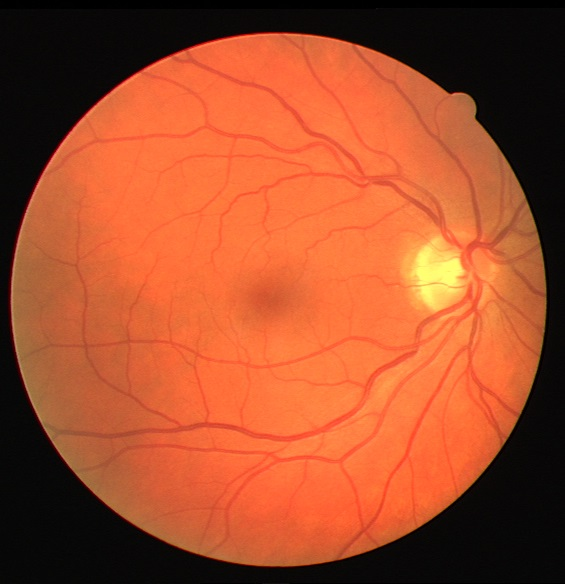
\includegraphics[width=4cm]{Graphics/train.jpg}
        \caption{Imágen de un ojo humano.}
    \end{subfigure}
    \begin{subfigure}{6cm}
        \centering
        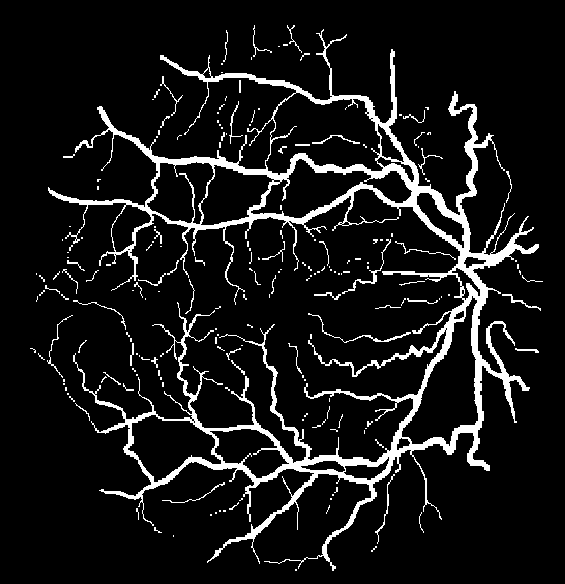
\includegraphics[width=4cm]{Graphics/mask.png}
        \caption{Vasos capilares del ojo.}
    \end{subfigure}
    \caption{Conjunto de imágenes de la base de datos de VesselNet.}
    \label{fig:vesselnet}
\end{figure}

\subsubsection{Filtro de alto contraste}

Se realizo un prepocesamiento a las imágenes para lograr difentes resultados. Uno de estos preprocesamientos fue el uso de un filtro de alto contraste para resaltar los vasos capilares en las imágenes de entrada. Esto fue implementado haciendo uso de la libreria de \script{opencv} de python. En la figura \ref{fig:high_contrast} se muestra el cambio visual que se obtiene al aplicar el filtro.

\begin{figure}[H]
    \centering
    \begin{subfigure}{6cm}
        \centering
        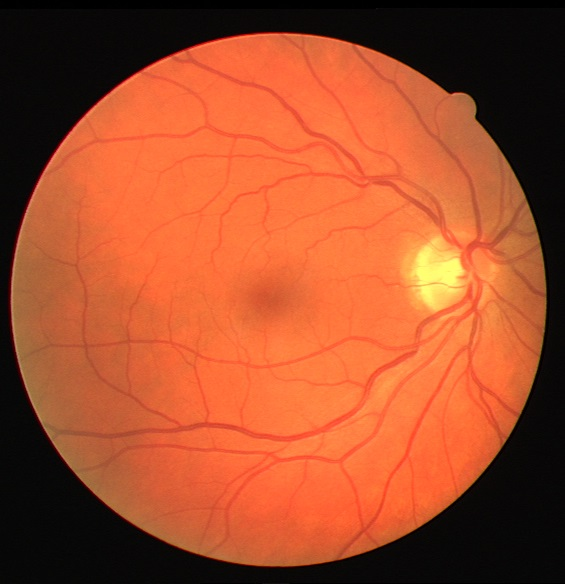
\includegraphics[width=4cm]{Graphics/train.jpg}
        \caption{Imágen original.}
    \end{subfigure}
    \begin{subfigure}{6cm}
        \centering
        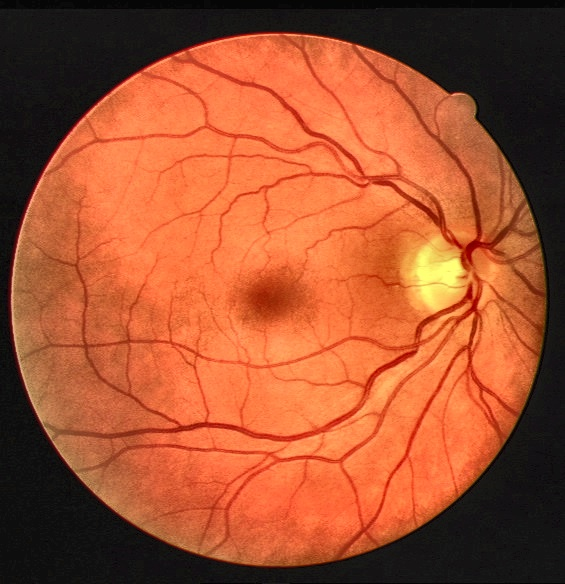
\includegraphics[width=4cm]{Graphics/high_contrast.jpg}
        \caption{Imágen con alto contraste.}
    \end{subfigure}
    \caption{Aplicación del alto contraste a la base de datos VesselNet.}
    \label{fig:high_contrast}
\end{figure}

\subsubsection{RGB a escala de grises}

A partir de las imágenes con alto contraste se transformaron estas imágenes para tenerlas en un espacio de grises. En la figura se muestra un ejemplo del resultado del realizar esta transforación.

\script{opencv} de python. En la figura \ref{fig:grayscale} se muestra el cambio visual que se obtiene al aplicar el filtro.

\begin{figure}[H]
    \centering
    \begin{subfigure}{6cm}
        \centering
        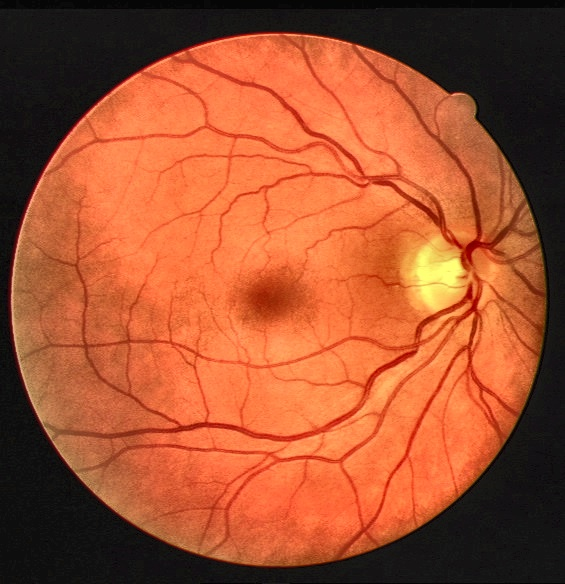
\includegraphics[width=4cm]{Graphics/high_contrast.jpg}
        \caption{Imágen con alto contraste.}
    \end{subfigure}
    \begin{subfigure}{6cm}
        \centering
        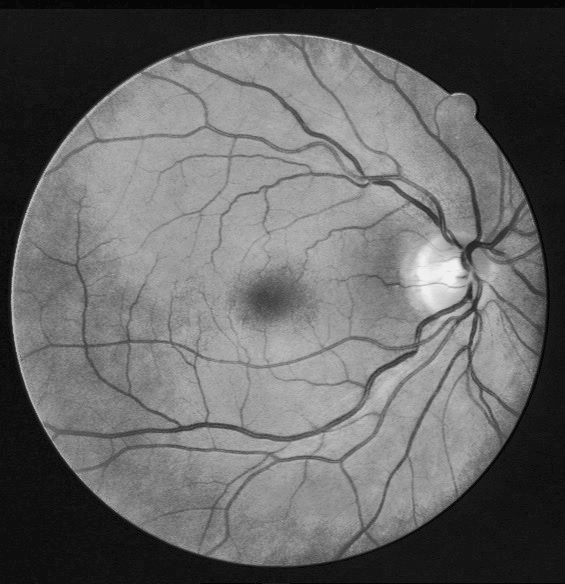
\includegraphics[width=4cm]{Graphics/grayscale.jpg}
        \caption{Imágen en escala de grises.}
    \end{subfigure}
    \caption{Transformación al espacio de grises.}
    \label{fig:grayscale}
\end{figure}

\subsubsection{Aumentación de imágenes}

Se realizaron diversas transformaciones para realizar una aumetación de los datos en el proceso de entrenamiento. Las transformaciones realizadas son las siguientes:

\begin{itemize}
    \item Rotaciones de no más de 90 grados.
    \item Desplazamientos de 0.3.
    \item Ampliación de la imegn de 0.3.
    \item Reflexiones de manera horizontal y vertical.
\end{itemize}